\chapter{Conclusion} \label{cha:conclusion}

The hypothesis \ref{hyp:modular} is right, source? Me.

\section{Modular Development}

In this thesis, we have shown that developing against a zero-core modular
architecture is trivial. By utilizing separation of concerns, a module developer
needs to only understand the feature they want to extend, or if it is an
entirely new feature, find out what has been done before.

Developing against an unstable \gls{api} is difficult, when developing a module
architecture, it is like an unstable \gls{api} when it is not \textit{mature},
e.g. when it does not have settled modules to develop against. Since this is
the case, there are a lot of issues with the existing modules, making the user
experience less than competing \gls{ide}s. Most of these are minors, and can be
fixed with some minor revisions to the existing modules, for instance, when
closing the \gls{ide}, unsaved changes are discarded, with no information given
to the user. Or how what project a user was working on, is not saved between
instances, so a user has to re-open the project they worked on. This is a side
effect of the development plan, and not the architecture. To fully test out this
architecture, it was thought that a wide range of modules should be implemented,
to quickly iron out issues with the implementation of the architecture, and to
figure out what functionality Tauri has, that we can expose, like the file
selection.
So not only were modules needed to cover the necessities to qualify as an
\gls{ide}, but they were also needed to \textit{test} the implementation. Not
having a developer dedicated to only implement modules, meant that module
development was usually dropped for other things. As every time a module where
worked on, it would eventually lead to a discovery, that the current \gls{api}
needed some change, which would enable the module feature to be easier
implemented. A concrete example of this, is the editor module.
An essential part of an editor, in an \gls{ide} at least, is being able to
utilize a \gls{lsp}. Most of the communication between a client and \gls{ls},
require information about \textit{where} the user is in the text. This
information is available in a \textit{textarea}-element, but some change to how
Events are sent were needed. In standard JavaScript development,
\textit{eventListeners} can be specific to the \gls{html}-element they are
applied to. The same is not possible in our \gls{api}, as Events are generic.
Instead we made Events gather information about the \gls{dom}-Event they were
triggered by, so in the case of \textit{click} attribute, we know the
\gls{dom}-event is of type \textit{MouseEvent}, which can give us some,
information. And if the \textit{target}, (a field on \textit{MouseEvent}) is an
instance of \textit{HtmlInputElement} or \textit{textarea}, we know that the
\textit{selectionStart} and \textit{value} field exist on the target. With
which, we can manually calculate the position of the click. Implementing this
meant adding a breaking change to the \gls{api}, which deprecated different
modules, so more time was spent on re-implementing them.

\subsection{Language Agnosticism}

Not really achieved, because we cannot syntactically translate between a
JavaScript Module and a Rust Module. This is due to the differences between the
utility libraries created for \gls{jsms} and \gls{rsms}. When \gls{jsms} modules
where created, they were primarily made for using existing JavaScript libraries,
to showcase this interoperability. So, much of the \gls{html} elements were
created using JavaScript, so the utility library primarily focused on this,
having builder pattern for creating \gls{html}. There is a similar builder
pattern in the Rust utility library, but it is not a one-to-one mapping, meaning
there are some semantic differences between two modules doing the same.

\subsection{Foreign Modules}

Languages like Gleam and PureScript, which compile directly to JavaScript can
be trivially added. But for languages that can target the C-\gls{abi}, this is
less trivial. This is because of how the core-\gls{ide} was designed. We decided
to use a \textit{Rust-y} approach, meaning we utilized many of the features that
made interoperability between the Rust-\gls{abi} and C-\gls{abi} more complex.
An example of this, can be found in the listing \ref{lst:value} and
\ref{lst:rsValue}, where we have the \textit{standard} value variant, and then
the \textit{C-safe} variant.

\begin{code}[H]
  \lstinputlisting
    [ language=Rust
    , caption={Value variant (Rust)}
    , label=lst:value
    , firstline=19
    , lastline=31
    ]{./core/src-tauri/core-std-lib/src/state/mod.rs}
\end{code}

\begin{code}[H]
  \lstinputlisting
    [ language=Rust
    , caption={C-safe value variant (Rust)}
    , label=lst:rsValue
    , firstline=16
    , lastline=21
    ]{./core/src-tauri/foreign-std-lib/src/state/rs\_state.rs}
\end{code}

Note the \textbf{\#[repr(C)]} macro attribute, and the two fields,
\textit{kind} and \textit{val}. The macro attribute specifies to the Rust
compiler that it should \textit{do what C does}. This is in regard to order,
size and alignment of fields of a structure. Since we cannot have the same enum
structure as we can in Rust, the work-around was an enum that specifies what
kind of value we are working with (\textit{val}), and a union, that holds the
specific value. A union in both C and Rust, has the same size in memory, as the
largest possible value it can store. In listing \ref{lst:rsValueUnion} we can
see this union. Accessing a field is inherently an \textit{unsafe} action, as we
cannot tell the compiler if the bytes we are reading are actually and integer,
or is a list of values. We can see this, as in the listing
\ref{lst:rsValueUnsafe}, on line three, we have to use the \textit{unsafe}
keyword in Rust, which essentially means the compiler cannot promise what we are
doing in this code block is \textit{valid}.

\begin{code}
  \lstinputlisting
    [ language=Rust
    , caption={Union used to hold the values the C-safe value can have (Rust)}
    , label=lst:rsValueUnion
    , firstline=134
    , lastline=144
    ]{./core/src-tauri/foreign-std-lib/src/state/rs\_state.rs}
\end{code}

\begin{code}
  \lstinputlisting
    [ language=Rust
    , caption={
      Accessing a value in the C-safe value variant is inherently unsafe
    }
    , label=lst:rsValueUnsafe
    , firstline=53
    , lastline=59
    , numbers=left
    , numberstyle=\tiny\color{gray}
    ]{./core/src-tauri/foreign-std-lib/src/state/rs\_state.rs}
\end{code}

\section{Making an IDE is hard}

An \gls{ide} has many features, which are needed to enhance the developer
experience. To achieve this, the modular approach enables future users to
enhance the application.

\begin{figure}
  \centering
  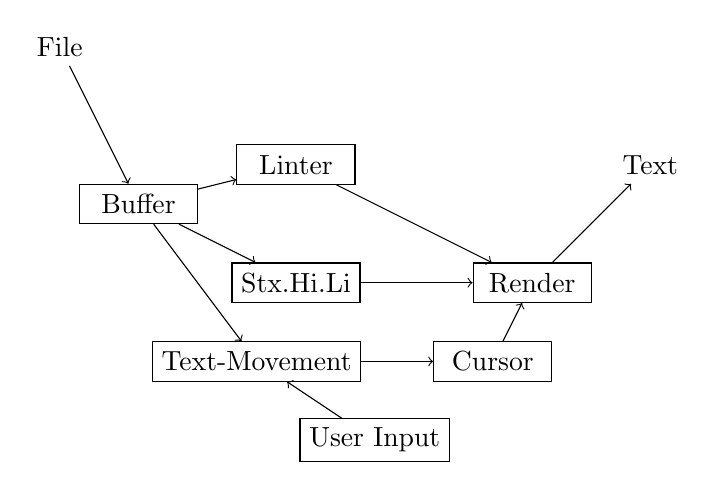
\begin{tikzpicture}
  % Nodes
  \node (file) [] at (-6, 3) {File};
  \node (parser) [rectangle, draw, minimum height=0.5cm, minimum width=1.5cm] at (-5, 1) {Buffer};
  \node (stxhili) [rectangle, draw, minimum height=0.5cm, minimum width=1.5cm] at (-3, 0) {Stx.Hi.Li};
  \node (text-movement) [rectangle, draw, minimum height=0.5cm, minimum width=1.5cm] at (-3.5, -1) {Text-Movement};
  \node (linter) [rectangle, draw, minimum height=0.5cm, minimum width=1.5cm] at (-3, 1.5) {Linter};
  \node (cursor) [rectangle, draw, minimum height=0.5cm, minimum width=1.5cm] at (-0.5, -1) {Cursor};
  \node (user-input) [rectangle, draw, minimum height=0.5cm, minimum width=1.5cm] at (-2, -2) {User Input};
  \node (render) [rectangle, draw, minimum height=0.5cm, minimum width=1.5cm] at (0, 0) {Render};
  \node (text) at (1.5, 1.5) {Text};
  % Arrow
  \draw[->] (file) -- (parser) node[midway, above] {};
  \draw[->] (parser) -- (stxhili) node[midway, above] {};
  \draw[->] (parser) -- (linter) node[midway, above] {};
  \draw[->] (parser) -- (text-movement) node[midway, above] {};
  \draw[<-] (render) -- (stxhili) node[midway, above] {};
  \draw[<-] (render) -- (linter) node[midway, above] {};
  \draw[<-] (cursor) -- (text-movement) node[midway, above] {};
  \draw[<-] (text-movement) -- (user-input) node[midway, above] {};
  \draw[->] (cursor) -- (render) node[midway, above] {};
  \draw[->] (render) -- (text) node[midway, above] {};
\end{tikzpicture}


  \caption{Text Editor Module Family}
  \label{fig:extendedModuleFamily}
\end{figure}

In the figure \ref{fig:extendedModuleFamily}, the \textit{cursor} is the place
at which text is placed when the user writes. If the user clicks someplace in
the document, the cursor \textit{jumps} to that place. If the user uses the
arrow-keys to move around, the cursor moves one character to left or right, or
one line up and down, depending on which arrow-key was pressed.

\section{Cons}

If you are the one developing every module, it get's very complex.

If you have a problem, and try to solve it with concurrency, now problems two
have you.
